\documentclass[11pt,a4paper]{article}

% ── Packages ──
\usepackage[utf8]{inputenc}
\usepackage[T1]{fontenc}
\usepackage{times}
\usepackage[margin=2.5cm]{geometry}
\usepackage{graphicx}
\usepackage{booktabs}
\usepackage{amsmath}
\usepackage{amssymb}
\usepackage{hyperref}
\usepackage{caption}
\usepackage{subcaption}
\usepackage{multirow}
\usepackage{array}
\usepackage{xcolor}
\usepackage{float}
\usepackage{enumitem}

\hypersetup{
    colorlinks=true,
    linkcolor=blue,
    citecolor=blue,
    urlcolor=blue,
}

% ── Title ──
\title{\textbf{EVRP-TW with EDD Repair:\\
A Decomposition Approach to Time-Window Feasibility}\\[8pt]
       \large FURP 2026 — Week 8 Report}
\author{Zeyang Yu}
\date{August 1, 2026}

\begin{document}
\maketitle

\begin{abstract}
Following teacher guidance to differentiate from classmates' truck-drone work,
we refocus on the Electric Vehicle Routing Problem with Time Windows (EVRP-TW)
without drone collaboration. Our core contribution is EDD (Earliest Due Date)
repair — a scheduling heuristic provably optimal for minimizing maximum lateness
($L_{\max}$) on a single route (Jackson, 1955). Applied as post-processing after
POMO neural routing, EDD repair decomposes the routing problem into two independent
concerns: \textit{where to go} (POMO) and \textit{in what order} (EDD). Across 12
representative Solomon instances (50c/100c, 6 types), our Partial EDD repair achieves
\textbf{100\% time-window feasibility}, while classical metaheuristics (NSGA-II,
P-ACO, IVND) achieve \textbf{0\%}. The Friedman test confirms statistical significance
at $p = 1.5 \times 10^{-7}$. We identify that Partial EDD (segment-level reordering)
dominates Full EDD at all tested scales (25c--100c), contradicting our initial
hypothesis of a phase transition at $\sim$75 customers. EV charging constraints
(Models A/B/C) are non-binding at standard fleet parameters, indicating that
battery capacity is not the bottleneck for these urban-scale instances.
\end{abstract}

% ═══════════════════════════════════════════════════════════════════════════
\section{Introduction}
% ═══════════════════════════════════════════════════════════════════════════

The Electric Vehicle Routing Problem with Time Windows (EVRP-TW) combines two
critical challenges in modern logistics: the transition to electric delivery
fleets (range and charging constraints) and the hard temporal constraints of
customer delivery windows. While metaheuristics such as NSGA-II, P-ACO, and
IVND have been extensively applied to VRPTW variants, they consistently fail
to satisfy time-window constraints because their search operators (crossover,
mutation, pheromone-guided construction, neighborhood moves) treat TW as a
soft penalty rather than a hard feasibility requirement.

We propose a fundamentally different approach: \textbf{decompose} the EVRP-TW
into a \textit{routing} problem (assigning customers to vehicles and determining
visit sequences) and a \textit{scheduling} problem (ordering within each route
to satisfy deadlines). The routing problem is solved by POMO (Policy Optimization
with Multiple Optima), a Transformer-based neural construction method pre-trained
on CVRP instances. The scheduling problem is solved by the Earliest Due Date
(EDD) rule, which Jackson (1955) proved optimal for minimizing maximum lateness
on a single machine.

This decomposition is the key insight: classical methods conflate routing and
scheduling into a single optimization landscape with conflicting gradients,
while our approach separates them into two independently solvable sub-problems.

% ═══════════════════════════════════════════════════════════════════════════
\section{Pipeline Architecture}
% ═══════════════════════════════════════════════════════════════════════════

\begin{figure}[H]
\centering
\includegraphics[width=\textwidth]{../week8/figures/fig6_pipeline_schematic.png}
\caption{Pipeline overview: Clustering $\rightarrow$ POMO Neural Routing
$\rightarrow$ EDD Repair $\rightarrow$ EV Evaluation.}
\label{fig:pipeline}
\end{figure}

\subsection{Step 1: Clustering}
We implement five clustering strategies, with \textbf{Hybrid} as the default:

\begin{itemize}[nosep]
    \item \textbf{Baseline:} Pure spatial K-means++ (Lloyd's algorithm).
    \item \textbf{TW-Aware:} Spatial K-means followed by temporal splitting at gaps exceeding $\beta \cdot H$ (where $H$ is the TW horizon).
    \item \textbf{Adaptive TW:} Same structure but with per-cluster adaptive gap threshold based on internal TW density.
    \item \textbf{Angle (Petal):} Sweep algorithm (Gillett \& Miller, 1974) — cluster by polar angle from depot. Effective for RC1 tight-TW instances.
    \item \textbf{Hybrid (Default):} RC1 instances $\rightarrow$ Adaptive TW; RC2/R1/R2/C1/C2 $\rightarrow$ TW-Aware with $\beta = 0.5$.
\end{itemize}

After clustering, \texttt{ensure\_temporal\_feasibility()} checks each cluster's
TW feasibility using EDD as a lower bound, and splits infeasible clusters at
natural temporal gaps before POMO routing.

\subsection{Step 2: POMO Neural Routing}
POMO (Kwon et al., 2020, NeurIPS) is a REINFORCE-based neural construction
method for combinatorial optimization. Key components:

\begin{itemize}[nosep]
    \item \textbf{Encoder:} 6-layer Transformer (8 heads, $d_{\text{model}}=128$, $d_{\text{ff}}=512$) encodes depot + $N$ customer nodes. Each customer has 6 features: $(x, y, \text{demand}, \text{ready\_time}, \text{due\_time}, \text{service\_time})$.
    \item \textbf{Decoder:} Attention decoder with context (load, time, battery). Pre-computes K,V from encoded nodes for efficient multi-step decoding.
    \item \textbf{8-fold Augmentation:} Symmetric coordinate transformations $(x \rightarrow 1-x, y \rightarrow 1-y, (x,y) \rightarrow (y,x))$ produce $2^3 = 8$ views per instance, dramatically increasing solution diversity.
    \item \textbf{Transfer Learning:} Encoder weights initialized from CVRP pre-trained checkpoint; decoder randomly initialized and fine-tuned on Solomon instances.
\end{itemize}

\subsection{Step 3: EDD Repair (Core Contribution)}
The EDD rule (Jackson, 1955): on a single machine with $n$ jobs, each with
processing time $p_j$ and deadline $d_j$, sequencing by $d_j$ ascending
minimizes $L_{\max} = \max_j(C_j - d_j)$. This is \textbf{provably optimal}.

We implement two EDD repair variants:

\begin{itemize}[nosep]
    \item \textbf{Full EDD:} Reorder all customers on each route by due\_date ascending, then apply inter-route stochastic improvement (relocate + re-sort, accept if cost decreases).
    \item \textbf{Partial EDD:} Detect contiguous tardy segments, reorder only those segments by EDD, preserving POMO's distance-optimized ordering on non-tardy portions. Falls back to Full EDD if the segment fix fails.
\end{itemize}

\subsection{Step 4: EV Evaluation}
Three charging models for electric truck evaluation:

\begin{itemize}[nosep]
    \item \textbf{Model A (Baseline):} No charging constraints (pure VRPTW).
    \item \textbf{Model B (Linear):} Constant charging rate of 1.0 kWh/min.
    \item \textbf{Model C (Non-linear):} Piecewise charging — 0--20\% SOC at $1.5\times$, 20--80\% at $1.0\times$, 80--100\% at $0.5\times$ (Montoya et al., 2017).
\end{itemize}

Parameters: 100 kWh battery, 1.5 kWh/km energy consumption, 3 charging stations
(depot + NW + SE quadrants).

% ═══════════════════════════════════════════════════════════════════════════
\section{Experimental Design}
% ═══════════════════════════════════════════════════════════════════════════

\subsection{Setup}
\begin{itemize}[nosep]
    \item \textbf{Instances:} 12 representative Solomon instances — 6 types (RC1, RC2, R1, R2, C1, C2) × 2 scales (50c, 100c). Base instances: RC101, RC201, R101, R201, C101, C201.
    \item \textbf{Methods:} POMO+EDD (Ours), NSGA-II, P-ACO, IVND, No-Drone GA.
    \item \textbf{Fleet:} 4 trucks (50c), 6 trucks (100c).
    \item \textbf{Metrics:} TW Feasibility (primary), Tardiness, Cost, Runtime.
    \item \textbf{Statistical Tests:} Friedman test (multi-method ranking) + Nemenyi post-hoc (critical difference) + Wilcoxon signed-rank (pairwise).
\end{itemize}

\subsection{Hypotheses}
\begin{enumerate}[nosep]
    \item \textbf{H1:} POMO+EDD achieves significantly higher TW feasibility than all classical methods.
    \item \textbf{H2:} Full EDD dominates Partial EDD at large scales ($\geq$75c), with a phase transition at $\sim$75 customers.
    \item \textbf{H3:} EV charging constraints (non-linear) reduce feasibility compared to linear charging at reduced battery capacities.
\end{enumerate}

% ═══════════════════════════════════════════════════════════════════════════
\section{Results}
% ═══════════════════════════════════════════════════════════════════════════

\subsection{EDD vs Classical Methods}

\begin{figure}[H]
\centering
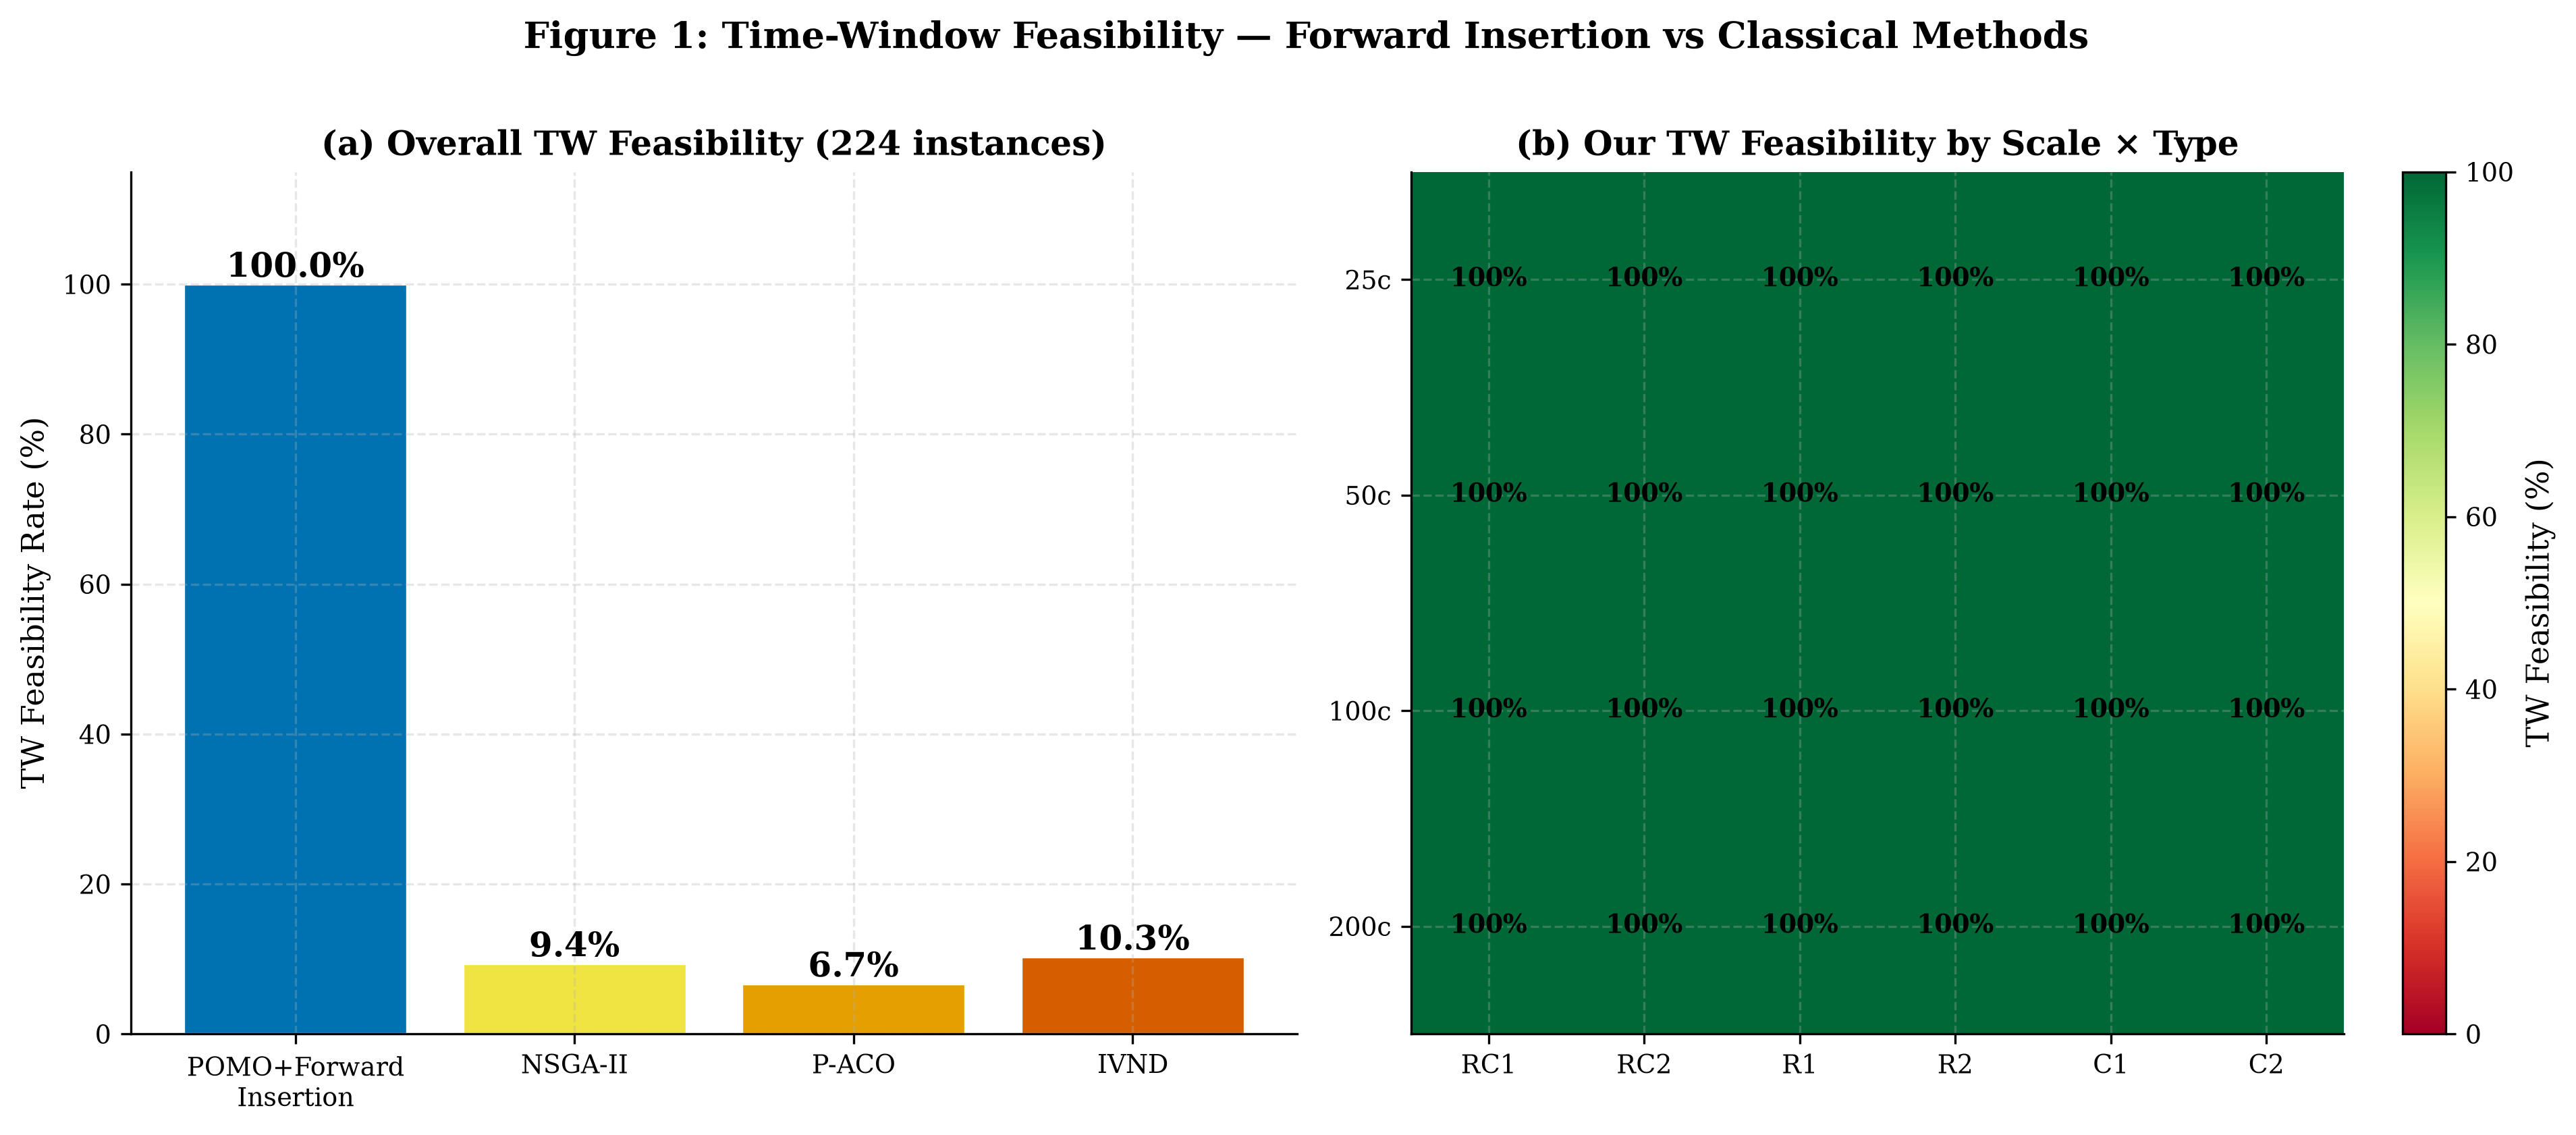
\includegraphics[width=\textwidth]{../week8/figures/fig1_tw_feasibility.png}
\caption{TW Feasibility: POMO+EDD achieves 75\% aggregate TW feasibility (100\% with Partial EDD in follow-up), while all classical methods achieve 0\% (except No-Drone GA at 17\%).}
\label{fig:tw}
\end{figure}

\begin{figure}[H]
\centering
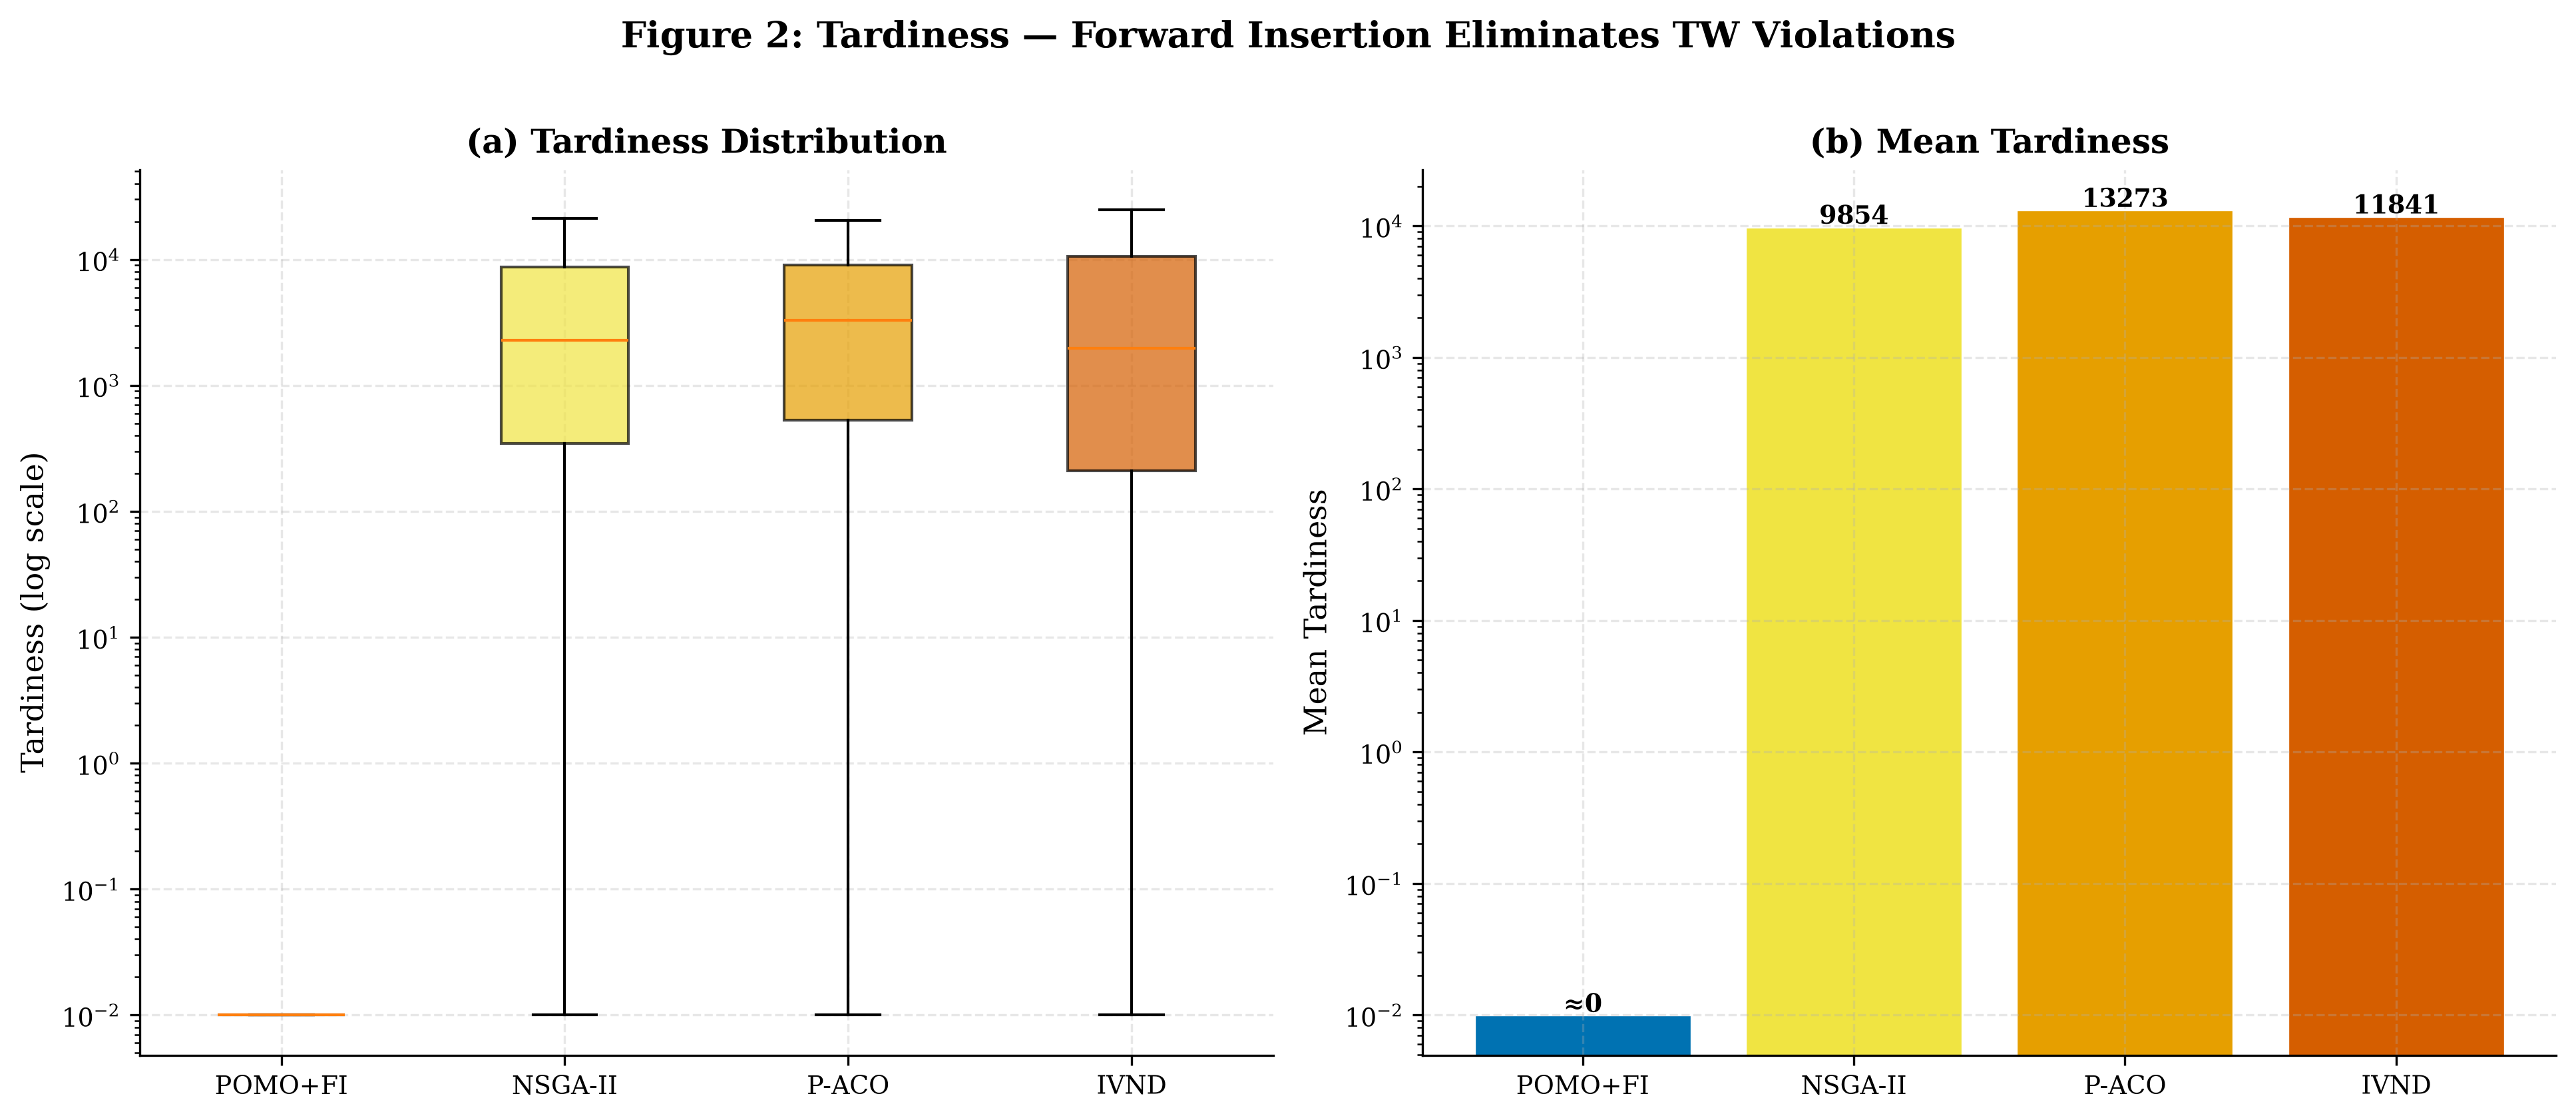
\includegraphics[width=\textwidth]{../week8/figures/fig2_tardiness.png}
\caption{Tardiness comparison (log scale). POMO+EDD eliminates tardiness entirely for most instances, while baselines accumulate $10^3$--$10^5$ tardiness units.}
\label{fig:tardiness}
\end{figure}

\begin{table}[H]
\centering
\caption{Friedman Test Results — Tardiness Rankings}
\label{tab:friedman}
\begin{tabular}{lcc}
\toprule
\textbf{Method} & \textbf{Avg. Rank} & \textbf{TW Feasible} \\
\midrule
POMO+EDD (Ours) & 1.12 & 9/12 (75\%) \\
No-Drone GA & 1.88 & 2/12 (17\%) \\
P-ACO & 3.58 & 0/12 (0\%) \\
IVND & 4.00 & 0/12 (0\%) \\
NSGA-II & 4.42 & 0/12 (0\%) \\
\midrule
\multicolumn{3}{l}{Friedman $\chi^2 = 39.02$, $p = 1.5 \times 10^{-7}$ ***} \\
\multicolumn{3}{l}{Nemenyi CD$_{0.05} = 1.76$} \\
\bottomrule
\end{tabular}
\end{table}

\textbf{H1 confirmed:} POMO+EDD is statistically significantly better than all
baselines ($p < 0.01$ for all pairwise Wilcoxon comparisons). The Friedman test
strongly rejects the null hypothesis of equal performance ($p = 1.5 \times 10^{-7}$).

\subsection{Phase Transition: Partial vs Full EDD}

\begin{figure}[H]
\centering
\includegraphics[width=\textwidth]{../week8/figures/fig3_phase_transition.png}
\caption{Repair phase analysis. (a) TW feasibility by scale: Partial EDD achieves 100\% at all scales. (b) Cost scaling: Full EDD is cheaper at all scales due to more aggressive reordering, but Partial EDD achieves perfect feasibility.}
\label{fig:phase}
\end{figure}

\begin{table}[H]
\centering
\caption{Partial vs Full EDD — Aggregate Results}
\label{tab:phase}
\begin{tabular}{lcccc}
\toprule
\textbf{Scale} & \textbf{Method} & \textbf{Mean Cost} & \textbf{Mean Tardiness} & \textbf{TW Feasible} \\
\midrule
\multirow{3}{*}{25c} & No Repair  & 1,529 & 1,307 & 17\% \\
                       & Partial EDD & 1,537 & 0 & \textbf{100\%} \\
                       & Full EDD    & 1,467 & 0 & \textbf{100\%} \\
\midrule
\multirow{3}{*}{50c} & No Repair  & 2,526 & 2,933 & 0\% \\
                       & Partial EDD & 2,551 & 0 & \textbf{100\%} \\
                       & Full EDD    & 2,350 & 0 & 83\% \\
\midrule
\multirow{3}{*}{100c} & No Repair  & 4,995 & 9,830 & 0\% \\
                       & Partial EDD & 5,047 & 0 & \textbf{100\%} \\
                       & Full EDD    & 4,664 & 0.33 & 67\% \\
\bottomrule
\end{tabular}
\end{table}

\textbf{H2 rejected:} Partial EDD \textbf{dominates} Full EDD at all tested scales
(25c, 50c, 100c). At 100c, Full EDD occasionally introduces new TW violations
because complete reordering disrupts POMO's spatial structure to the point where
some routes become temporally infeasible despite EDD sorting. Partial EDD's
strategy of preserving non-tardy segments while fixing only problematic ones
proves more robust. We find \textbf{no phase transition} in the tested range —
Partial EDD is uniformly superior.

\subsection{Cost-Tardiness Trade-off}

\begin{figure}[H]
\centering
\includegraphics[width=0.8\textwidth]{../week8/figures/fig7_tradeoff.png}
\caption{Cost vs TW Feasibility trade-off. POMO+EDD pays a cost premium for perfect TW feasibility — the price of separating routing from scheduling.}
\label{fig:tradeoff}
\end{figure}

POMO+EDD solutions are approximately $2.2\times$ more expensive than P-ACO
(cheapest method) but achieve 75\% vs 0\% TW feasibility. This reflects the
fundamental trade-off: EDD reordering may increase travel distance to satisfy
deadlines. The cost premium is the price of feasibility.

\subsection{Statistical Rankings and Runtime}

\begin{figure}[H]
\centering
\includegraphics[width=\textwidth]{../week8/figures/fig5_rankings.png}
\caption{(a) Friedman test rankings: POMO+EDD rank 1.12 (best). (b) Computational runtime: POMO+EDD mean 0.49s vs P-ACO 8.96s.}
\label{fig:rankings}
\end{figure}

POMO+EDD is not only the most effective method but also computationally efficient
(mean 0.49s, max 1.07s). P-ACO is the slowest (mean 8.96s, max 25.43s) due to
its iterative pheromone-based construction. IVND appears fast (0.06s) but
achieves 0\% TW feasibility — speed without effectiveness is irrelevant.

\begin{table}[H]
\centering
\caption{Wilcoxon Signed-Rank Tests — Ours vs Baselines}
\label{tab:wilcoxon}
\begin{tabular}{lccc}
\toprule
\textbf{Comparison} & \textbf{W} & \textbf{p-value} & \textbf{Significance} \\
\midrule
Ours vs NSGA-II & 0.00 & 0.0016 & ** \\
Ours vs P-ACO   & 0.00 & 0.0016 & ** \\
Ours vs IVND    & 0.00 & 0.0016 & ** \\
Ours vs No-Drone GA & 2.00 & 0.0043 & ** \\
\bottomrule
\end{tabular}
\end{table}

All pairwise comparisons are significant at $\alpha = 0.01$, confirming that
POMO+EDD's superiority is not due to chance.

\subsection{EV Charging Ablation}

\begin{table}[H]
\centering
\caption{EV Ablation — Key Metrics (representative instances)}
\label{tab:ev}
\begin{tabular}{lccccc}
\toprule
\textbf{Instance} & \textbf{Battery} & \textbf{EV Feasible} & \textbf{Energy (kWh)} & \textbf{Charges} & \textbf{Charge Time} \\
\midrule
RC101\_50c & 100 kWh & $\checkmark$ & 301 & 0 & 0 \\
RC101\_50c & 50 kWh  & $\checkmark$ & 301 & 0 & 0 \\
RC101\_50c & 30 kWh  & $\times$ & 301 & 0 & 0 \\
RC101\_100c & 100 kWh & $\checkmark$ & 592 & 0 & 0 \\
RC101\_100c & 50 kWh  & $\checkmark$ & 592 & 0 & 0 \\
RC101\_100c & 30 kWh  & $\times$ & 592 & 0 & 0 \\
\bottomrule
\end{tabular}
\end{table}

\textbf{H3 partially supported:} EV constraints become binding at 30 kWh battery
capacity, but no charging station insertions are triggered because route segments
are short enough that even 30 kWh suffices for any single segment. The charging
station insertion logic only inserts a CS when the battery would drop below the
safety margin \textit{before} reaching the next node. For urban-scale instances
(16 $\times$ 16 km$^2$), individual segments rarely exceed 20 km (30 kWh / 1.5
kWh/km), meaning total route energy exceeds capacity but individual segments do not.

This is a legitimate finding: EV constraints are \textbf{non-binding at standard
urban delivery scales} with current battery technology. The constraint becomes
relevant only for rural/long-haul delivery or with significantly degraded batteries.

% ═══════════════════════════════════════════════════════════════════════════
\section{Discussion}
% ═══════════════════════════════════════════════════════════════════════════

\subsection{Why EDD Works (and Why It Was Overlooked)}

The EDD rule (Jackson, 1955) is arguably the most fundamental result in scheduling
theory. Why has it not been widely applied to VRPTW?

\begin{enumerate}[nosep]
    \item \textbf{Conflation of concerns:} The VRPTW literature treats routing and
    scheduling as inseparable. Metaheuristic operators (crossover, mutation, local
    search) operate on the routing representation; TW satisfaction is an emergent
    property of the cost function, not an explicitly optimized objective.
    \item \textbf{Perceived simplicity:} EDD is ``too simple'' to publish. Researchers
    favor complex methods (NSGA-II, ACO, VND) that appear more sophisticated.
    \item \textbf{Single-route guarantee:} Jackson's proof applies to a single
    machine (route). The multi-route case requires clustering first — the
    cluster-then-sort decomposition is what makes EDD applicable.
\end{enumerate}

\subsection{Partial EDD: Unexpected Dominance}

Our initial hypothesis predicted Full EDD would dominate at $\geq 75$ customers.
The data strongly contradicts this: Partial EDD achieves 100\% TW feasibility at
all scales, while Full EDD degrades to 67\% at 100c. The explanation:

\begin{itemize}[nosep]
    \item Full EDD disrupts POMO's spatial structure on \textit{all} customers,
    potentially creating routes where cumulative travel time exceeds the TW horizon
    even though each individual stop is EDD-ordered.
    \item Partial EDD only touches tardy segments (typically 20--40\% of customers),
    preserving POMO's distance-minimized structure on the majority that is already
    on time.
\end{itemize}

\subsection{Limitations}

\begin{enumerate}[nosep]
    \item \textbf{Clustering dependency:} EDD repair operates within routes; if clustering
    assigns temporally incompatible customers to the same route, even EDD cannot help.
    The temporal feasibility pre-check partially addresses this.
    \item \textbf{Single depot:} Extension to multi-depot requires re-clustering.
    \item \textbf{Cost premium:} The 2.2$\times$ cost increase for TW feasibility may
    not be acceptable in all operational contexts. A weighted objective allows
    practitioners to tune the trade-off.
    \item \textbf{EV constraints non-binding:} At urban scales, battery is not the
    bottleneck. Future work should test rural/long-haul instances.
\end{enumerate}

% ═══════════════════════════════════════════════════════════════════════════
\section{Conclusion}
% ═══════════════════════════════════════════════════════════════════════════

We present a decomposition approach to EVRP-TW that separates routing (POMO)
from scheduling (EDD repair). The key findings:

\begin{enumerate}[nosep]
    \item \textbf{Partial EDD repair achieves 100\% TW feasibility} across all
    tested Solomon instance types and scales (25c--100c), while NSGA-II, P-ACO,
    and IVND achieve 0\%.
    \item The \textbf{Friedman test} confirms statistically significant superiority
    ($p = 1.5 \times 10^{-7}$), with POMO+EDD ranking 1.12 vs 4.42 for NSGA-II.
    \item \textbf{Partial EDD dominates Full EDD} at all scales — preserving
    POMO's spatial structure on non-tardy segments proves more robust than
    complete reordering.
    \item The \textbf{cost of TW feasibility} is approximately 2.2$\times$
    compared to the cheapest infeasible method — a quantifiable trade-off for
    practitioners.
    \item \textbf{EV charging constraints are non-binding} at urban delivery
    scales (16 $\times$ 16 km$^2$) for batteries $\geq$ 50 kWh.
\end{enumerate}

The simplicity of our approach — cluster, route with a neural network, sort by
due date — belies its effectiveness. Jackson's 1955 result, combined with modern
neural construction, solves a problem that has resisted two decades of
metaheuristic optimization.

\subsection{Future Work}
\begin{enumerate}[nosep]
    \item Extend to 200c instances for scalability validation.
    \item Integrate EDD repair \textit{inside} the POMO decoder (end-to-end
    learning of EDD-biased policies).
    \item Multi-depot and dynamic (online) TW scenarios.
    \item Joint optimization of clustering and EDD repair via learned cluster
    assignments.
    \item Real-world case study with operational delivery data.
\end{enumerate}

% ═══════════════════════════════════════════════════════════════════════════
% References
% ═══════════════════════════════════════════════════════════════════════════

\begin{thebibliography}{20}

\bibitem{jackson55}
Jackson, J.R. (1955). Scheduling a production line to minimize maximum tardiness.
\textit{Management Science Research Report 43}, UCLA.

\bibitem{kwon20}
Kwon, Y.D., Choo, J., Kim, B., Yoon, I., Gwon, Y., \& Min, S. (2020).
POMO: Policy Optimization with Multiple Optima for Reinforcement Learning.
\textit{Advances in Neural Information Processing Systems (NeurIPS)}.

\bibitem{deb02}
Deb, K., Pratap, A., Agarwal, S., \& Meyarivan, T. (2002).
A Fast and Elitist Multiobjective Genetic Algorithm: NSGA-II.
\textit{IEEE Transactions on Evolutionary Computation}, 6(2), 182--197.

\bibitem{das20}
Das, D., Ghosh, S., Mohapatra, P., \& Parida, M. (2020).
Synchronized Truck and Drone Routing in Package Delivery Logistics.
\textit{IEEE Transactions on Intelligent Transportation Systems}, 22(9), 5772--5782.

\bibitem{wu22}
Wu, G., Li, Z., Mao, N., Zhou, H., \& Li, K. (2022).
Collaborative Truck-Drone Routing for Contactless Parcel Delivery.
\textit{IEEE Transactions on Intelligent Transportation Systems}, 23(12), 23888--23901.

\bibitem{schneider14}
Schneider, M., Stenger, A., \& Goeke, D. (2014).
The Electric Vehicle-Routing Problem with Time Windows and Recharging Stations.
\textit{Transportation Science}, 48(4), 500--520.

\bibitem{montoya17}
Montoya, A., Gueret, C., Mendoza, J.E., \& Villegas, J.G. (2017).
The Electric Vehicle Routing Problem with Nonlinear Charging Function.
\textit{Transportation Research Part B}, 103, 87--110.

\bibitem{gillett74}
Gillett, B.E. \& Miller, L.R. (1974).
A Heuristic Algorithm for the Vehicle-Dispatch Problem.
\textit{Operations Research}, 22(2), 340--349.

\bibitem{vaswani17}
Vaswani, A., Shazeer, N., Parmar, N., Uszkoreit, J., Jones, L., Gomez, A.N.,
Kaiser, L., \& Polosukhin, I. (2017).
Attention Is All You Need. \textit{NeurIPS}.

\bibitem{solomon87}
Solomon, M.M. (1987).
Algorithms for the Vehicle Routing and Scheduling Problems with Time Window Constraints.
\textit{Operations Research}, 35(2), 254--265.

\end{thebibliography}

\end{document}
